

\documentclass[a4paper,11pt]{article}
\usepackage{amsmath,amssymb,amsfonts,amsthm, mathrsfs}
\usepackage{tikz}
\usepackage [utf8x] {inputenc}
\usepackage [T2A] {fontenc} 
\usepackage[russian]{babel}
\usepackage{cmap} 
\RequirePackage{caption}
\DeclareCaptionLabelSeparator{defffis}{. }
\captionsetup{justification=centering,labelsep=defffis}

\usepackage[mathscr]{eucal}
\usepackage{braket}
% Так ссылки в PDF будут активны
\usepackage[unicode]{hyperref}
\usepackage{mathtools}


% вы сможете вставлять картинки командой \includegraphics[width=0.7\textwidth]{ИМЯ ФАЙЛА}
% получается подключать, как минимум, файлы .pdf, .jpg, .png.
\usepackage{graphicx}
% Если вы хотите явно указать поля:
\usepackage[margin=1in]{geometry}
% Или если вы хотите задать поля менее явно (чем больше DIV, тем больше места под текст):
% \usepackage[DIV=10]{typearea}

\usepackage{fancyhdr}

\newcommand{\bbR}{\mathbb R}%теперь вместо длинной команды \mathbb R (множество вещественных чисел) можно писать короткую запись \bbR. Вместо \bbR вы можете вписать любую строчку букв, которая начинается с '\'.
\newcommand{\eps}{\varepsilon}
\newcommand{\bbN}{\mathbb N}
\newcommand{\dif}{\mathrm{d}}
\usepackage[cal=boondox]{mathalfa} %todo

\pagestyle{fancy}
\makeatletter % сделать "@" "буквой", а не "спецсимволом" - можно использовать "служебные" команды, содержащие @ в названии
\fancyhead[L]{\footnotesize}%Это будет написано вверху страницы слева
\fancyhead[R]{\footnotesize Karamyshev Anton}
%\fancyfoot[L]{\footnotesize \@author}%имя автора будет написано внизу страницы слева
\fancyfoot[R]{\thepage}%номер страницы —- внизу справа
\fancyfoot[C]{}%по центру внизу страницы пусто.
\renewcommand{\maketitle}{%
	\noindent{\bfseries\scshape\large\@title\ \mdseries\upshape}\par
	\noindent {\large\itshape\@author}
	\vskip 2ex}
\makeatother
\def\dd#1#2{\frac{\partial#1}{\partial#2}}

\usepackage{xcolor}


\bibliographystyle{acm}% Choose Phys. Rev. style for bibliography

\author{Karamyshev}

\begin{document}

\textbf{Abstract} --- Мы предлагаем четырехкубитный квантовый протокол распределения ключей, базирующийся на измерении двух состояния Белла. Кубиты объединяются в единый блок, передаваемый от отправителя к получателю в каждом сообщении. Шифрование здесь разработано путем случайной группировки четырех отдельных кубитов в две новые пары, такой механизм также является одним из способов обнаружить подслушивающее устройство в канале. В конечном счете, приемник случайным образом проверяет полученный блок при помощи двух измерений состояний Белла. Из сравнения информации о группировке этих четырех кубитов обе стороны соединения могут обнаружить нелегального пользователя в канале. В предложенном протоколе приемник обрабатывает блок мгновенно во время получения, что является эффективным способом преодоления ультракороткого времени хранения квантового состояния.



\section{История и предпосылки}

Квантовое распределение ключей (англ.: Quantum Key Distribution, QKD) — метод передачи ключа, который использует квантовые явления для гарантии безопасной связи. Этот метод позволяет двум сторонам, соединенным по открытому каналу связи, создать общий случайный ключ, который известен только им, и использовать его для шифрования и расшифрования сообщений.


В настоящее время предложено довольно много работ по данной тематике. Самый первый протокол QKD был предложен Беннеттом и Брассардом в 1984 году. Данный протокол получил название BB84 и базировался на использовании двух взаимно несмещенных состояний поляризации фотонов \cite{BB84}. Авторами был описан способ распределения случайного секретного ключа между Алисой и Бобом. 
 
Позднее Экерт предложил другой протокол QKD \cite{E91}, названный E91, основанный на парадоксе Эйнштейна-Подольского-Розена \cite{EPR}. После этого были теоретически предложены и экспериментально реализованы различные протоколы QKD, например, базирующиеся на однофотонных \cite{liang2015simple} и множественных состояниях \cite{fourstate}. Среди этих работ для переноса информации широко используются фотоны, поскольку ими легко манипулировать и они передают информацию со скоростью света.

Новый виток в развитии QKD связан с использованием состояний Белла \cite{EPR}.
В качестве квантового канала состояние Белла было впервые предложено в \cite{Gao} и подтверждено как максимально запутанное состояние двухкубитной квантовой системы. Кроме того, по сравнению с другими мультикубитными состояниями (состояния W \cite{W}, GHZ \cite{GHZ} и кластерные состояния \cite{cluster}), состояние Белла легче всего реализовать с помощью нелинейного процесса, описанного в  \cite{twophotons}. 

В основополагающей работе \cite{Gao} две стороны разделяют секретный ключ, сравнивая форму начального состояния Белла и результат измерения состояния Белла после квантовой перекрутки %todo.
Затем \cite{nine} повысил общую эффективность коммуникации до 100\% по сравнению с достигнутыми 50\% в \cite{Gao}. В \cite{ten} представлен первый аутентифицированный полуквантовый протокол распределения ключей без использования аутентифицированных классических каналов, основанный на состояниях Белла.

В недавней работе \cite{base} было предложено усовершенствование \cite{ten} для предотвращения подслушивания с более низким коэффициентом ошибок при подтверждении сообщений, а также с более быстрым обнаружением битов ключа, основанных на четырехкубитном состоянии, которое состоит из двух пар состояний Белла. Дальнейшая речь пойдёт о протоколе, представленном в \cite{base}.




В нашем протоколе каждый раз подготавливается группа состоящая из четырёх кубитов, которая затем передаётся от отправителя к получателю. Приемник производит квантовое измерение состояния сразу после получения кубитов. По сравнению с двусторонними протоколами, в которых квантовое состояние должно сохраняться до завершения передачи в \cite{Gao} и \cite{nine}, наш протокол может преодолеть проблему времени ультракороткой когерентности квантовых состояний. Каждые четыре кубита образуют единый блок для передачи информации от отправителя к получателю в каждом сообщении. Четыре выхода посылаются отправителем в случайном порядке и принимаются получателем в некотором случайном групповом измерении. Наши расчеты показывают, что коэффициент ошибок при выходе составляет 4.17\%, что ниже, чем 46.875\% в \cite{eleven}. Кроме того, только 11 бит необходимы для обнаружения подслушивающего устройства в нашем QKD протоколе, которое меньше 72 бит в BB84 протоколе \cite{BB84} с тем же уровнем безопасности.
\section{QKD PROTOCOL BASED ON FOUR-QUBIT STATES}

\subsection{Квантовый канал на основе состояний Белла}
[8] и [9] предложили два протокола QKD, которые используют состояния Белла, распределенные между отправителем и получателем. В их протоколах две пары состояний Bell разделены между двумя сертифицированными сторонами связи. Отправитель и получатель хранят по два кубита, запутанные друг с другом. После одновременного измерения состояния Белла (BSM) с двух сторон реализуется квантовая запутанность уже между четырьмя кубитами.

Если давать более формальное описание, то можно обозначить четыре кубита двух состояний Белла как $P_1$, $P_2$, $P_3$ и $P_4$. Запутанность имеет место между $P_1$ и $P_2$, а также между $P_3$ и $P_4$. После измерения состояний Белла с обеих сторон запутанными оказываются $P_1$ и $P_3$, $P_2$ и $P_4$ соответственно. Однако обеим сторонам все равно необходимо хранить свои кубиты во время всего процесса коммуникации, и хранить кубиты в нужном состоянии довольно сложно в современном мире.


Учитывая ультракороткое время хранения кубитов, был предложен новый протокол QKD с четырехкубитной конфигурацией, состоящей из двух пар состояний Белла, выраженных уравнением (1). Группа состояний из четырех кубитов каждый раз подготавливается для незамедлительной отправки Бобу для измерения. Основное отличие от [8] и [9] заключается в том, что отправитель посылает сразу все кубиты приемнику, а приемник производит измерение квантового состояния сразу же после получения всей партии кубитов. Это односторонний процесс. Обеим сторонам не нужно продолжительное время хранить кубиты, так как кубиты измеряются незамедлительно после получения.

\begin{table}
	\centering
	\caption{\label{tab:1}Соответствие состояний Белла и бинарной случайной последовательности.}
	\begin{tabular}{ |c||c||c| }
		\hline
		$(P_1, P_3)$ & $(P_1, P_3)$ & $\mathcal{K}$ \\ \hline
		$\ket{\phi^+}$ & $\ket{\phi^-}$ & 00 \\ 
		$\ket{\phi^-}$ & $\ket{\phi^+}$ & 01 \\ 
		$\ket{\psi^+}$ & $\ket{\psi^-}$ & 10 \\ 
		$\ket{\psi^-}$ & $\ket{\psi^+}$ & 11 \\ 
		\hline
	\end{tabular}
\end{table}

\begin{table}
	\centering
	\caption{\label{tab:2}Различные группировки кубитов для Боба.}
	\begin{tabular}{ |c||c||c| }
		\hline
		Bob's grouping & Verdict & Announced number \\ \hline
		$(P_1, P_3)\&(P_2, P_4)$ & Right & 1 \\
		$(P_1, P_2)\&(P_3, P_4)$ & Wrong & 0 \\
		$(P_1, P_4)\&(P_2, P_3)$ & Wrong & 0 \\
		\hline
	\end{tabular}
	
\end{table}



\begin{equation*}
\ket{\mathcal{C}}_{1234} = \ket{\phi^-}_{12} \otimes \ket{\phi^+}_{34}
= \dfrac{1}{2} \Big(\ket{\phi^+}_{13} \ket{\phi^-}_{24} + 
 					\ket{\phi^-}_{13} \ket{\phi^+}_{24} +
 					\ket{\psi^+}_{13} \ket{\psi^-}_{24} +
 					\ket{\psi^-}_{13} \ket{\psi^+}_{24} \Big),
\end{equation*}

где индексы $1$, $2$, $3$ и $4$ обозначают 4 связанных кубита. Состояние Белла выражается следующим образом:

\begin{equation*}
\ket{\phi^{\pm}} = \dfrac{1}{\sqrt2}\big(\ket{00} \pm \ket{11} \big), \quad
\ket{\psi^{\pm}} = \dfrac{1}{\sqrt2}\big(\ket{01} \pm \ket{10} \big).
\end{equation*}


Из (1) видно, что состояние становится суперпозицией четырех состояний, что означает, что мы можем получить четыре различных результата с помощью комбинаций состояний Белла. Обратим внимание, что уравнение (1) представляет только один особый случай, две другие формы с различными группировками кубитов для сравнения показаны в Таблице II. Вкратце, существует три формы случайной группировки этих четырех кубитов, из которых только уравнение (1) определено как правильное. Это основной метод шифрования информации во время коммуникации. Предлагаемый протокол показан на Рис. 1, где Алиса и Боб являются законными отправителем и приемником соответственно.

\subsection{Алгоритм формирования ключей}

\begin{itemize}

\item \textit{Шаг 1. Подготовка состояний.} Алиса подготавливает одну из комбинаций четырёхкубитных состояний, представленных в уравнении (1). Каждая такая группа состоит из четырёх кубитов $P_\gamma, \gamma \in \{1,2,3,4\}$. Для такого способа кодирования информация ключа $\mathcal{K}$ в соответствии с состоянием Белла представлена в таблице 1. Алиса запоминает текущее состоянии кубитов и соответствующую информацию ключа $\mathcal{K}$.

\item \textit{Шаг 2. Распределение кубитов.} Согласно договорённости Алиса знает, что рассматриваемые четыре кубита сгруппированы как $\{(P_1, P_3), (P_2, P_4)\}$, а Боб -- нет. Алиса случайным образом переставляет эти четыре кубита и отправляет их Бобу по квантовому каналу.

\item \textit{Шаг 3. Измерение состояний Белла.} Боб принимает отправленные ему кубиты и случайным образом разбивает их на две части. После чего он выполняет измерение состояний Белла на этих двух частях и отправляет полученные результаты Алисе по классическому каналу. Различные варианты группировки четырёх кубитов для Боба приведены в таблице $2$.

\item \textit{Шаг 4. Сравнение результатов.} Алиса принимает результаты Боба и сравнивает их с сохранённой информацией о $P_\gamma$. Если Алиса увидит совпадение, она объявит по классическому каналу $'1'$ и весь процесс коммуникации может перейти к шагу $5$ или вернуться на шаг $1$. Если же совпадения не случится, она объявит $'0'$ и процесс коммуникации начнётся сначала с шага $1$ или оборвётся. 

\item \textit{Шаг 5. Получение согласованных ключей.} После нескольких итераций шагов c $1$ по $4$ Алиса и Боб получают двоичную последовательность, которая представляет собой некоторый необработанный ключ $\mathcal{R}$. Под $\mathcal{R}_A$ и $\mathcal{R}_B$ будем понимать необработанные ключи Алисы и Боба соответственно. Алиса случайным образом выбирает части $\mathcal{R}_A$ и собирает из них своей согласованный ключ $\mathcal{C}_A$, после чего объявляет позиции выбранных частей по классическому каналу. Затем Боб согласно этим позициям выбирает свой согласованный ключ $\mathcal{C}_B$ из ключа $\mathcal{R}_B$.

\item \textit{Шаг 6. Усиление конфиденциальности.} Из полученного набора битов $\mathcal{C}_B$ Боб выбирает некоторые в качестве битов чётности $\mathcal{D}_B$ и объявляет $\mathcal{D}_B$ вместе с их соответствующими позициями. Аналогичным образом Алиса выбирает свой набор $\mathcal{D}_A$ и сравнивает его с полученным $\mathcal{D}_B$. Если процент битовых ошибок в таком сравнении меньше некоторого наперёд заданного порога, то соединение может считаться безопасным и процесс коммуникации может перейти к следующему шагу $7$; если нет, то необходимо вернуться на шаг $1$ или же окончательно оборвать связь.

\item \textit{Шаг 7. Формирование окончательных ключей.} На последнем шаге окончательно выбираются ключи $\mathcal{R'}_A$ и $\mathcal{R'}_B$, которые будут использоваться для шифрования в дальнейшем процессе коммуникации. Теоретически, в идеальном случае должно получиться $\mathcal{R'}_A$ = $\mathcal{R'}_B$, где $\mathcal{R'}_A$ --- это необработанный ключ $\mathcal{R}_A$ исключая биты $\mathcal{C}_A$, аналогичное верно для $\mathcal{R'}_B$.
\end{itemize}

\subsection{Анализ доли ошибочных кубитов}

Мы видим, что существуют три различных способа группировок кубитов, представленных в таблице 2. Мы условились, что первая группировка является правильной, а две остальных --- неправильными. Учитывая, что каждая из трёх группировок получается равновероятно, вероятность правильной группировки по Бобу равна $\frac{1}{3}$. Если в канале нет подслушивающего устройства, то вероятность ошибки $\varepsilon_0$ может быть рассчитана следующим образом.

(1) Пусть Боб случайным образом получил неправильную группировку кубитов, например $\{(P_1 , P_2), (P_3 , P_4)\}$.

\begin{equation*}
\ket{\mathcal{C}}_{1234} = \dfrac{1}{2} \Big(\ket{0000} + \ket{0011}
 + \ket{1100} + \ket{1111} \Big)_{1234} = 2 \Big(\ket{\phi^-}_{12} \ket{\phi^+}_{34}\Big).
\end{equation*}

В этом случае, из всех комбинаций состояний Белла он получит только $\ket{\phi^-}_{12} \ket{\phi^+}_{34}$. Согласно таблице $1$ получит правильную бинарную последовательность $\mathcal{K} = 01$ c вероятностью $\frac{1}{4}$.

(2) Рассмотрим другой случай неправильной группировки $\{(P_1, P_4), (P_2, P_3)\}$.

\begin{align*}
\ket{\mathcal{C}}_{1234} = \dfrac{1}{2} \Big(\ket{0000} + \ket{0011}
&+ \ket{1100} + \ket{1111} \Big)_{1234} \nonumber\\
 = \dfrac{1}{2} \Big(
\ket{\phi^+}_{14} \ket{\phi^-}_{23} + \ket{\phi^-}_{14} \ket{\phi^+}_{23} &+ 
\ket{\psi^+}_{14} \ket{\psi^-}_{23} + \ket{\psi^-}_{14} \ket{\psi^+}_{23} \Big).
\end{align*}

Измеряя состояния Белла, он может получить любую из перечисленных комбинаций состояний Белла: $\{\ket{\phi^+}, \ket{\phi^-}\}$, $\{\ket{\phi^-}, \ket{\phi^+}\}$, $\{\ket{\psi^+}, \ket{\psi^-}\}$ и $\{\ket{\psi^-}, \ket{\psi^+}\}$. Как результат, согласно таблице $1$ Боб получит правильную бинарную случайную последовательность $\mathcal{K}$ с вероятностью $\frac{4}{4} = 1$. Ещё раз отметим, что это происходит при неправильной группировке.

%китайцы ебанаты
Таким образом, результаты измерений состояний Белла могут быть частично верными в первом случае или полностью верными во втором случае. Как результат, в случае неправильной группировки Боб может получить правильную двоичную случайную последовательность с вероятностью $\frac{1}{2} \cdot \frac{1}{4} + \frac{1}{2} \cdot \frac{4}{4} = \frac{5}{8}$. Следовательно, доля ошибочных кубитов $\varepsilon_0$ равна:

\begin{equation*}
\varepsilon_0 = 1 - \Big(\dfrac{1}{3} + \dfrac{5}{8}\Big) = \dfrac{1}{24} = 0.0417.
\end{equation*}

Ещё раз отметим, что если Боб выберет правильную группировку с вероятностью $\frac{1}{3}$, он может получить правильную двоичную случайную последовательность с вероятностью $1$. В конечном счёте, порог для предложенного алгоритма может быть установлен равным $4.17\%$.

\section{SECURITY ANALYSES}
In this section, we analyze the security of our protocol under two major attacks: the intercept-resend attack and the Trojan Horse attack. Meanwhile, we assume the existence of
an eavesdropper Eve in the communication channel.

\subsection{The intercept-resend attack}
The eavesdropper Eve can interact and resend a new four-qubit state to Bob so that he can acquire the information of the state. In this case, Eve plays the same role as Bob does in the communication. He can group the four-qubit state and measure it with Bell bases.

After step $2$ of our protocol, the four qubits sent by Alice will transmit through the communication channel. Let’s assume that Eve intercepts these four qubits and processes
them in the same way as Bob does. Then, Eve resends his decoy four qubits to Bob. Let us discuss the different cases of the communication between Eve and Bob.

($1$) Eve chooses the right grouping and acquires the right measurement results. Bob simultaneously chooses the right grouping. Now, there are three parties, Alice, Bob and Eve
in the communication. There is a probability of $p_1$ that Eve can successfully filch the information,

\begin{equation*}
 p_1 = \Big(\dfrac{1}{3} \cdot 1 \Big)_{Eve} \times  \Big(\dfrac{1}{3} \cdot 1 \Big)_{Bob} = \dfrac{1}{9}.
\end{equation*}

(2) Similarly, Eve can divide the qubits and obtain the measurement results correctly. Then, he sends the right decoy four-qubit state to Bob. After receiving them, Bob chooses a wrong grouping but yields a right measurement result.

However, this group of state will be abandoned since in the comparison stage Alice and Bob can detect the wrong grouping.

\begin{equation*}
p_2 = \Big(\dfrac{1}{3}\cdot 1 \Big)_{Eve} \times \Big(\dfrac{2}{3}\cdot \dfrac{1}{4} + 
\dfrac{2}{3} \cdot \dfrac{5}{8} \Big)_{Bob} = \dfrac{14}{72}.
\end{equation*}

(3) Eve chooses a wrong grouping but he gets a right measurement result while Bob chooses a right grouping.

\begin{equation*}
p_3 = \Big(\dfrac{2}{3}\cdot \dfrac{1}{4} + 
\dfrac{2}{3} \cdot \dfrac{5}{8} \Big)_{Eve} \times \Big( \dfrac{1}{3}\cdot 1 \Big)_{Bob} = \dfrac{14}{72}.
\end{equation*}

(4) In the same way, Eve transmits the decoy state with a wrong grouping but Bob gets the right results. Meanwhile, Bob divides this decoy four-qubit state into wrong groups but
obtain the right measurement result. In this case, the qubits will be abandoned because of the wrong grouping of Bob.

\begin{equation*}
p_4 = Big(\dfrac{2}{3}\cdot \dfrac{1}{4} + 
\dfrac{2}{3} \cdot \dfrac{5}{8} \Big)_{Eve} \times \Big(\dfrac{2}{3}\cdot \dfrac{1}{4} + 
\dfrac{2}{3} \cdot \dfrac{5}{8} \Big)_{Bob} = \dfrac{49}{144}.
\end{equation*}

In conclusion, there is a probability that Bob gets a wrong measurement result, i.e., the qubit error rate with existence of eavesdropper in our protocol can be calculated as (8).

\begin{equation*}
\varepsilon_e = 1 - \Big(\dfrac{1}{9} + \dfrac{14}{72} + \dfrac{14}{72} + \dfrac{49}{144} \Big) = \dfrac{23}{144} = 0.1597.
\end{equation*}

Suppose Alice and Bob need to compare n bits of binary random sequence to detect Eve with the probability of $p_d = 0.999999999$ with

\begin{equation*}
p_d = 1 - (1-\varepsilon_e) = 1 - \Big(\dfrac{23}{144} \Big)^n.
\end{equation*}

We can find a minimum value of $n = 11$ from equation (9). On the other hand, in BB84 protocol, Alice and Bob need to compare $n = 72$ bits to detect Eve with the same probability. From the aforementioned analyses, we can calculate the mutual information between Alice, Bob and Eve. The mutual information between Alice and Bob is

\begin{equation*}
I(A; B) = 1 - [-(1-\varepsilon_0)log(1-\varepsilon_0) - \varepsilon_0 log \varepsilon_0] = 0.7501.
\end{equation*}

The mutual information between Alice and Eve is 
\begin{equation*}
I(A; E) = 1 - [-(1-\varepsilon_e)log(1-\varepsilon_e) - \varepsilon_e log \varepsilon_e] = 0.3664.
\end{equation*}

Therefore, the communication is secure since $I(A; B) > I(A; E)$. Furthermore, $I(A; B)$ in our protocol is greater than $I' (A; B) = 0.1887$ bit in BB84 protocol.
The theoretical secret key rate is
\begin{equation*}
R = I(A; B) - I(A; E) = 0.7501 - 0.3664 = 0.3837 > 0.
\end{equation*}

So, the binary random bits can be distilled after Alice and Bob perform key reconciliation and privacy amplification on the final key $\mathcal{R}'_A$ and $\mathcal{R}'_B$. The transmission distance $\mathcal{l}$ of the secret key is given by the qubit error rate $\varepsilon$ [12], which is:

\begin{equation*}
\varepsilon = \dfrac{\mu \eta 10^{- \frac{\alpha \mathcal{l}}{10}}}{\mu \eta 10^{- \frac{\alpha \mathcal{l}}{10}} + 2P_e}, 
\end{equation*}

where $\mu = 4$ is the averaged qubit flux leaving from Alice, $10^{- \frac{\alpha \mathcal{l}}{10}}$ represents the fiber attenuation through distance $\mathcal{l}$,
$\eta$ is the detection efficiency. Here, we set the channel loss to be $\alpha = 0.2$ and
$\alpha = 0.5$. Referring to [12], $P_e = 8.5 \cdot 10^{−7}$ is the probability of an error count per clock cycle. We set the values of $\eta$ to be $0.2$, $0.5$ and $0.99$.
Figure 2 shows the relation between $\mathcal{l}$ (km) and the qubit error rate $\varepsilon$. We can see that $\mathcal{l}$ decreases with the increase of the channel loss. Meanwhile, the higher the detection efficiency of the communication $\eta$ is, the larger the qubit error rate $\varepsilon$ is. From Fig. 2, we can infer that there exists a further distance when $\varepsilon_e$ = 0.0417 which is the qubit error rate in our protocol.

\cite{base}


\subsection{Атака троянского коня}

Атака троянского коня \cite{trojan,trojan2, trojan4}, подразумевает, что система QKD может быть взломана Евой путем отправки яркого света в квантовый канал и анализа обратного отражения. Ева использует вспомогательный источник, модулирует его и анализирует обратно рассеянный сигнал с помощью детектора. Как правило \cite{trojan}, схема обнаружения истинного сигнала основана на особенностях вспомогательного источника, например, на его фазе. Еве необходимо удалить часть истинного сигнала, и затем компенсировать введенные потери с помощью улучшения квантового канала. Следовательно, Еве нужно подготовить канал, который имеет меньшее затухание, чем изначальный квантовый канал. Если это выполнено, Ева может измерить перехваченное состояние с помощью квантовой памяти.

\begin{figure}[h]
	\center{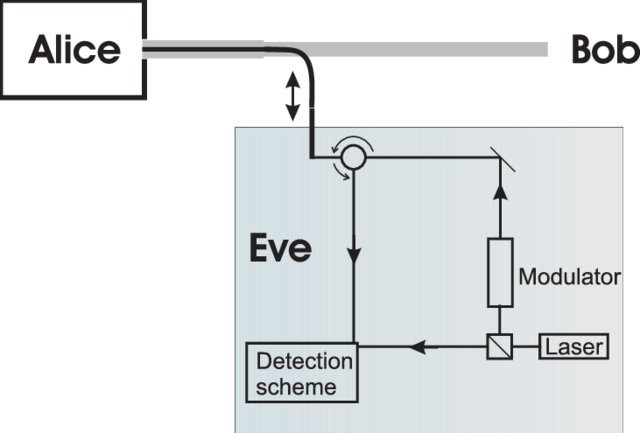
\includegraphics[width=0.5\linewidth]{trojan.jpg}}
	\label{ris:image1}
\end{figure}


При атаке Троянского Коня известно измерение \cite{trojan, trojan3}, которое максимизирует собственную информацию Евы, т.е. информационный выигрыш:

\begin{equation*}
\mathcal{I}_{Eve}(|\alpha|^2) = 1 - h(p),
\end{equation*}

где $p = \frac{1}{2} \big(\sqrt{1 - |\braket{\alpha, 0 | 0, \alpha}|^2 } \big) \approx \frac{1 + \sqrt2 |\alpha|}{2}$, $(p) = -p\log_2(p) - (1-p)\log_2(p)$, $|\alpha|^2$ обозначает номер фотона Евы.

Раскладывая выражение для собственной информации Евы в ряд Тейлора получим:

\begin{align*}
\mathcal{I}_{Eve}(|\alpha|^2) &\approx 1 + 
\Big( \frac{1 + \sqrt2 |\alpha|}{2} \Big) \log_2 \Big(\frac{1 + \sqrt2 |\alpha|}{2}\Big) + \Big( \frac{1 - \sqrt2 |\alpha|}{2} \Big) \log_2 \Big(\frac{1 - \sqrt2 |\alpha]|}{2}\Big) = \nonumber \\
&= 1 - 1 + \frac{(\sqrt2 |\alpha|)^2}{\log4} + \frac{(\sqrt2 |\alpha|)^4}{6\log4} + \mathcal{O}(|\alpha|^6) = \frac{|\alpha|^2}{\log2} + \mathcal{O}(|\alpha|^4).
\end{align*}

Согласно полученному выражению и границам, представленным в \cite{trojan} мы можем заключить \cite{base}, что $\max\limits_{|\alpha|^2} \big\{\mathcal{I}_{Eve} (|\alpha|^2) \big\} < \mathcal{I}(A; B)$. Следовательно, атака троянского коня может
быть предотвращена в рассматриваемом протоколе.


\section{Numerical Appendix}

\begin{equation*}
\ket{\phi^{\pm}} = \dfrac{1}{\sqrt2}\big(\ket{00} \pm \ket{11} \big), \quad
\ket{\psi^{\pm}} = \dfrac{1}{\sqrt2}\big(\ket{01} \pm \ket{10} \big).
\end{equation*}



\begin{align*}
\ket{\mathcal{C}}_{1234} = \ket{\phi^-}_{12} \otimes \ket{\phi^+}_{34}
= \dfrac{1}{2} \big(\ket{00}_{12} - \ket{11}_{12} \big) \otimes \big( \ket{00}_{34} + \ket{11}_{34} \big) = \nonumber \\
= \dfrac{1}{2} \big(\ket{0000} + \ket{0011} - \ket{1100} - \ket{1111}\big)_{1234} =
\end{align*}

\begin{align*}
\ket{\mathcal{C}}_{1234} = \dfrac{1}{2} \Big(\ket{\phi^+}_{13} \ket{\phi^-}_{24} + 
\ket{\phi^-}_{13} \ket{\phi^+}_{24} +
\ket{\psi^+}_{13} \ket{\psi^-}_{24} +
\ket{\psi^-}_{13} \ket{\psi^+}_{24} \Big) = \nonumber \\
\end{align*}

\begin{align*}
\ket{\phi^+}_{m} \ket{\phi^-}_{n} = \dfrac{1}{2} \big(\ket{00}_m \ket{00}_n - \ket{00}_m \ket{11}_n + \ket{11}_m \ket{00}_n - \ket{11}_m \ket{11}_n \big) \nonumber \\
\ket{\phi^-}_{m} \ket{\phi^+}_{n} = \dfrac{1}{2} \big(\ket{00}_m \ket{00}_n + \ket{00}_m \ket{11}_n - \ket{11}_m \ket{00}_n - \ket{11}_m \ket{11}_n \big) \nonumber \\
\ket{\psi^+}_{m} \ket{\psi^-}_{n} = \dfrac{1}{2} \big(\ket{01}_m \ket{01}_n - \ket{01}_m \ket{10}_n + \ket{10}_m \ket{01}_n - \ket{10}_m \ket{10}_n \big)
\nonumber \\
\ket{\psi^-}_{m} \ket{\psi^+}_{n} = \dfrac{1}{2} \big(\ket{01}_m \ket{01}_n + \ket{01}_m \ket{10}_n - \ket{10}_m \ket{01}_n - \ket{10}_m \ket{10}_n \big)
\end{align*}

\bibliography{ru}

\end{document}

